%%%%%%%%%%%%%%%%%%%%%%%%%%%%%% -*- Mode: Latex -*- %%%%%%%%%%%%%%%%%%%%%%%%%%%%
%% 05-01-results.tex -- Thesis: Priority Ranked Inspection
%% Author          : Aaron A. Kagawa
%% Created On      : Mon April 14 11:52:28 2005
%% Last Modified By: Aaron Kagawa
%% Last Modified On: Wed Jul  6 11:48:40 2005
%% RCS: $Id$
%%%%%%%%%%%%%%%%%%%%%%%%%%%%%%%%%%%%%%%%%%%%%%%%%%%%%%%%%%%%%%%%%%%%%%%%%%%%%%
%%   Copyright (C) 2004 Aaron A. Kagawa
%%%%%%%%%%%%%%%%%%%%%%%%%%%%%%%%%%%%%%%%%%%%%%%%%%%%%%%%%%%%%%%%%%%%%%%%%%%%%%%


\chapter{Results}
\label{chapter:results}
This chapter presents the results of this research. The procedure I used in
my exploratory study is explained in Chapter \ref{chapter:evaluation}. In
this study, I tested three of my thesis claims. The following list states
my thesis claims and their associated results:

\begin{description}

\item[Thesis Claim 1:] Inspecting MINI documents will generate more
  high-severity defects than inspecting LINI documents.
\begin{itemize}
\item[-] The results show supporting evidence for Thesis Claim 1.
\end{itemize}

\item[Thesis Claim 2:] PRI can enhance the volunteer-based document
  selection process.
\begin{itemize}
\item[-] The results show supporting evidence for Thesis Claim 2.
\end{itemize}

\item[Thesis Claim 3:] PRI can identify documents that need to be inspected
  that are not typically identified by volunteering.
\begin{itemize}
\item[-] The results are inconclusive for Thesis Claim 3. 
\end{itemize}
\end{description}

The sections of this chapter are organized in the following manner. In
Section \ref{section:limitations}, I revisit some of the limitations that
hinder the results of this study. In Section \ref{section:inspections}, I
summarize the results of the conducted inspections. In Section
\ref{section:terminology}, I explain a few terms that will help explain the
results. In the next three sections, Sections \ref{section:claim1},
\ref{section:claim2}, and \ref{section:claim3}, I provide supporting
evidence for my thesis claims.  These three sections are organized by
presenting the strongest evidence first. Therefore, the order is Thesis
Claim 1 (Section \ref{section:claim1}), Thesis Claim 2 (Section
\ref{section:claim2}), and finally Thesis Claim 3 (Section
\ref{section:claim3}). In Appendix
\ref{appendix:chapter:pre-selection-questionnaire-results}, I present the
raw data results from the Pre-Selection-Questionnaire. In Appendix
\ref{appendix:chapter:inspection-results}, I present the raw data results
from the inspections and Post-Inspection-Questionnaire.


\section{Limitations Revisited}
\label{section:limitations}
As explained in the previous chapter, there are many limitations associated
with the study of this research. Most notably is the absence of sufficient
inspection resources within the CSDL organization, during the time period
of my study, to thoroughly inspect a wide spectrum of MINI and LINI
documents to determine the correctness of the PRI rankings. As expected,
this limitation of the exploratory study also limits the results presented
in this chapter. Unfortunately, this limitation has affected my ability to
come to a definitive answer to my third thesis claim, which states that PRI
can identify documents that need to be inspected that are not typically
identified by volunteering.

\section{Inspections}
\label{section:inspections}
Throughout the duration of this research, starting in September 2004 till
June 2005, I led CSDL in 20 different inspections. On average 5 to 6 CSDL
members participated in each of the inspections. In addition, with an
estimated cost of 2 hours\footnote{According to CSDL's inspection process,
  each member should spend about an hour individually inspecting the
  document. Another hour is spent in the inspection meeting.} per
inspection per member, CSDL spent about 220 hours dedicated to inspection.
Although 220 hours seems substantial, I've estimated that we would require
about 3,500 hours to inspect the entire Hackystat system, which would be a
very unrealistic demand on CSDL's resources for this research. Therefore,
as I've previously stated, my study investigated a small percentage of the
system in hopes that a cross-section provides adequate and acceptable
results.

%%Furthermore, I am the first researcher to evaluate of CSDL's current
%%inspection process and use of Jupiter. Therefore, some of the results
%%presented in this section were a little surprising.

Ten of the twenty inspections were designated to be part of the methodology
used evaluate my thesis claims. Unfortunately, one of the 10 inspections
that were designated for the study, namely Inspection 10, had to be
excluded from the results, because the code that was inspected was written
entirely in C++ and could not be ranked by PRI \footnote{I allowed
  developers to select any code they were most concerned about, therefore
  in this instance the inspection could not be used in my study.}.

\begin{table}[!h]
  \begin{center}
    \caption{All Inspection - Results by Severity}
    \label{tab:inspection-results}
    \begin{tabular}{|p{2.0cm}|p{1.5cm}|p{1.5cm}|p{1.5cm}|p{1.5cm}|p{1.5cm}|p{1.5cm}|} \hline
{\bf Inspection} & {\bf Critical} & {\bf Major} 
& {\bf Normal} & {\bf Minor} & {\bf Trivial} & {\bf Total} \\ \hline
 8 & 1 & 7 & 11& 2 & 3 & 24 \\ \hline
 9 &   & 16& 13& 4 & 4 & 37 \\ \hline
11 & 1 & 14& 13& 14& 1 & 43 \\ \hline
12 &   & 13& 12& 6 &   & 31 \\ \hline
13 & 1 & 7 & 1 & 2 &   & 11 \\ \hline
14 & 1 & 13& 12&   &   & 26 \\ \hline
15 &   & 1 & 6 & 2 & 1 & 10 \\ \hline
16 &   & 3 & 4 & 3 &   & 10 \\ \hline
17 &   & 7 & 6 & 1 & 3 & 17 \\ \hline
{\bf Total} & {\bf 4} & {\bf 81} & {\bf 78} & {\bf 34} & {\bf 12} & {\bf
  209} \\ \hline
{\bf Percentage} & {\bf 1.9 \%} & {\bf 38.8 \%} & {\bf 37.3 \%} & {\bf 16.3 
  \%} & {\bf 5.7 \%} &  \\ \hline 
    \end{tabular}
  \end{center}
\end{table}

Table \ref{tab:inspection-results} displays a general overview of the
inspection results for each inspection conducted under the study procedure.
Taking a closer look at the inspection results shows that the inspections
have found a considerable amount of valid defects. Furthermore, notice that
a large percentage, 40.2 percent to be exact, of the defects are
high-severity defects. High-severity defects are defined as defects with a
severity equal to ``Critical'' or ``Major'' and with a resolution not equal
to ``Invalid Won't Fix'' and ``Valid Duplicate''. See Section
\ref{section:evaluation-subjects} for a discussion on how defects are
collected using CSDL's inspection process and the Jupiter tool.

Using the Type property associated with the valid defects provides a
different view of the inspection results. Table
\ref{tab:inspection-results-type} shows the results listed by different
defects types provided by Jupiter. Note that the types ``Missing'',
``Irrelevant'', and ``Other'' were omitted from this table, because the use
of these types were very limited, accounting for only 12 of the 209
defects. According to these results, Coding Standards and Program Logic
account for more than half the valid defects discovered in CSDL's
inspections. Although not officially stated in CSDL's inspection process
and is largely based on the developers' subjective opinion, Coding
Standards defects are generally reserved for defects resulting in defects
in code formatting, variable and method naming conventions, Javadoc
documentation, and the alike. Program Logic defects are generally problems
associated with Object-Oriented design, algorithmic, calculation errors,
and other problems associated with the actual functionality of the software
code.

\begin{table}[!h]
  \begin{center}
    \caption{All Inspection - Results by Type}
    \label{tab:inspection-results-type}
    \begin{tabular}{|p{2.0cm}|p{1.7cm}|p{1.5cm}|p{1.7cm}|p{1.4cm}|p{1.4cm}|p{1.5cm}|}  \hline   
\small{} {\bf Inspection} & \small{}{\bf Coding Standards} & 
\small{}{\bf Program Logic} & \small{} {\bf Optimi- zation} & 
\small{}{\bf Usability} & \small{} {\bf Clarity} & 
\small{} {\bf Suggestion} \\ \hline

 8 & 10& 6 & 1 & 2 & 5 &      \\ \hline
 9 & 9 & 13& 3 & 4 & 3 & 4    \\ \hline
11 & 22& 7 & 3 & 2 &   & 7    \\ \hline
12 & 14& 4 & 1 & 4 & 6 & 2    \\ \hline
13 & 5 & 6 &   &   &   &      \\ \hline
14 & 9 & 4 & 1 & 8 & 1 & 2    \\ \hline
15 & 6 & 2 &   &   & 1 &      \\ \hline
16 &   &   & 2 & 1 & 3 & 3    \\ \hline
17 & 2 & 2 & 5 &   & 2 &      \\ \hline

{\bf Total} & {\bf 77} & {\bf 44} & {\bf 16} & {\bf 21} & {\bf 21} & {\bf
  18} \\ \hline

{\bf Total} & {\bf 36.8 \%} & {\bf 21.1 \%} & {\bf 7.7 \%} & {\bf 10.0 \%} &
{\bf 10.0 \%} & {\bf 8.6 \%} \\ \hline

    \end{tabular}
  \end{center}
\end{table}

Further analyzing the Type and Severity properties of the defects shows
that Program Logic defects are of more concern than any other type.
According to Table \ref{tab:inspection-results-type-severity} and also
shown in Figure \ref{fig:inspection-results-7}, Program Logic defects
account for the majority of the high-severity defects. On the other hand,
Coding Standard defects account for the majority of the low-severity
defects. This result indicates that Program Logic defects are generally
high-severity problems. Therefore, an inspection that finds more Program
Logic defects generally also has a larger number of high-severity defects.

\begin{table}[!h]
  \begin{center}
    \caption{All Inspections - Results by Type and Severity}
    \label{tab:inspection-results-type-severity}
    \begin{tabular}{|p{2.0cm}|p{1.7cm}|p{1.5cm}|p{1.7cm}|p{1.4cm}|p{1.4cm}|p{1.5cm}|}  \hline   
\small{} & \small{}{\bf Coding Standards} & 
\small{}{\bf Program Logic} & \small{} {\bf Optimi- zation} & 
\small{}{\bf Usability} & \small{} {\bf Clarity} & 
\small{} {\bf Suggestion} \\ \hline

{\bf Critical} &   & 3 &   & 1 &   &      \\ \hline
{\bf Major}    & 13& 28& 11& 8 & 6 & 10    \\ \hline
{\bf Normal}   & 31& 12& 4 & 12& 13& 4    \\ \hline
{\bf Minor}    & 24& 1 & 1 &   & 1 & 4    \\ \hline
{\bf Trivial}  & 9 &   &   &   & 1 &      \\ \hline

{\bf Total} & {\bf 77} & {\bf 44} & {\bf 16} & {\bf 21} & {\bf 21} & {\bf
  18} \\ \hline
    \end{tabular}
  \end{center}
\end{table}

\begin{figure}[!h]
  \centering
  \includegraphics[width=1.0\textwidth]{figs/Results/inspection-results-7.eps}
  \caption{All Inspections - Results by Severity and Type}
  \label{fig:inspection-results-7}
\end{figure}

\clearpage
\section{Result Terminology}
\label{section:terminology}
Throughout the rest of this chapter, I will be using the terms
\textit{MINI-p, MINI-d, and LINI-p}. These terms represent three different
groups of packages that were inspected in this study. I will use these
three different groups of packages to explain the results and charts
presented in the following sections.

\begin{itemize}
\item[-] \textbf{MINI-p} represents inspections 8 and 9.  According to the
  PRI rankings generated by the Hackystat PRI Extension, these inspections
  were conducted on MINI packages. In addition, according to the
  developers' rankings, these were also MINI packages. The developer
  rankings were obtained in the Pre-Selection-Questionnaire.
\item[-] \textbf{MINI-d} represents inspections 11, 12, and 14. According
  to the developers' rankings, these inspections were conducted on MINI
  packages. The developer rankings were obtained in the
  Pre-Selection-Questionnaire. However, according to the PRI rankings
  generated by the Hackystat PRI Extension, these packages were LINI. This
  group is interesting, because the developers and PRI ranking disagreed. 
\item[-] \textbf{LINI-p} represents inspections 13, 15, 16, and 17.
  According to the PRI rankings generated by the Hackystat PRI Extension,
  these inspections were conducted on LINI packages. However, no developer
  rankings were obtained for these packages.
\end{itemize}

In addition, to distinguish between the two different methods used in this
study to rank packages, I will use the terms \textit{dMINI, dLINI, pMINI,
  and pLINI}. These terms distinguish between packages that were ranked by
the Hackystat PRI Extension and packages that were ranked by the
developers. The terms \textit{MINI and LINI} will still be used with
discussing the general meaning of \textit{More In Need of Inspection} and
\textit{Less In Need of Inspection}.

\begin{itemize}
\item[-] \textbf{dMINI and dLINI} represents the MINI and LINI packages 
  according to the developers' opinion. 
\item[-] \textbf{pMINI and pLINI} represents the MINI and LINI packages
  according to the Hackystat PRI Extension. 
\end{itemize}


\clearpage
\section{Thesis Claim 1}
\label{section:claim1}
\noindent Claim: \textit{MINI documents will generate more high-severity
  defects than LINI documents.} \newline 

The results presented in this section will provide evidence to support this
claim. The supporting evidence for this claim is apparent in four separate
results. The first supporting evidence is the results shown in Figure
\ref{fig:inspection-results-1}, which charts the total number of defects
and the number of high-severity defects. Second, the results shown in
Figure \ref{fig:post-inspection-1}, which charts the responses from the
Post-Inspection-Questionnaire. Third, the results shown in Figure
\ref{fig:inspection-results-3}, which charts the various defect types.
Fourth, the results shown in Figure \ref{fig:inspection-results-5}, which
charts the average review active time from all participants. Each of these
results is independent supporting evidence that provides varying levels of
support for Thesis Claim 1.

\subsection{Inspection Results by Severity}
Figure \ref{fig:inspection-results-1} shows the results of the Severity
property associated with the defects found in the inspections conducted on
the three different groups, MINI-p, MINI-d, and LINI-p.

\begin{figure}[!h]
  \centering
  \includegraphics[width=1.0\textwidth]{figs/Results/inspection-results-1.eps}
  \caption{Inspection Results - Severity}
  \label{fig:inspection-results-1}
\end{figure}

Figure \ref{fig:inspection-results-average-1} provides the average number
of defects and average number of high-severity defects in the MINI-p,
MINI-d, and the LINI-p groups. The results in the Figure show that on
average the MINI-p group generated about 18 more defects of any severity
compared to the LINI-p group. Furthermore, on average the MINI-p group have
generated about 8 more high-severity defects than the LINI-p group. This
result provides supporting evidence for Thesis Claim 1. The fact that the
MINI-p and MINI-d groups generated more defects than the LINI-p group
provides supporting evidence that the Hackystat PRI Extension and
developers can identify MINI documents. However, in the case of the MINI-d
group, where the developers indicated a MINI ranking but PRI indicated a
LINI ranking, the results provide evidence that the developers were correct
and the PRI ranking was incorrect. In other words, this data suggests the
presence of possible 'false negatives' by PRI. More inspections and
evaluations are needed to determine if PRI can correctly rank the packages
in the MINI-d group.

\begin{figure}[!h]
  \centering
  \includegraphics[width=1.0\textwidth]{figs/Results/inspection-results-average-1.eps}
  \caption{Inspection Results - Average Severity}
  \label{fig:inspection-results-average-1}
\end{figure}

Figure \ref{fig:inspection-results-2} shows the percentage of high-severity
defects over total defects for each of the inspections. Figure
\ref{fig:inspection-results-average-1-percent} shows the average percentage
for the MINI-p, MINI-d, and LINI-p groups. According to Figure
\ref{fig:inspection-results-average-1-percent}, there does not appear to be
a significant difference between the three groups in terms of the
percentage of high-severity defects. However, it is my contention that this
percentage is not useful in determining the correctness of the MINI and
LINI determination, because the number of total defects does not stay
constant throughout each inspection. For example, Inspection 13 has the
highest percentage, however referring back to Figure
\ref{fig:inspection-results-1} will show that this inspection contained the
third lowest number of total defects and fourth lowest number of
high-severity defects. Therefore, I believe that this percentage should not
be used to compare the results of individual inspections.

\begin{figure}[!htb]
  \centering
  \includegraphics[width=1.0\textwidth]{figs/Results/inspection-results-2.eps}
  \caption{Inspection Results - Severity Percentage}
  \label{fig:inspection-results-2}
\end{figure}

\begin{figure}[!htb]
  \centering
  \includegraphics[width=1.0\textwidth]{figs/Results/inspection-results-average-1-percent.eps}
  \caption{Inspection Results - Average Severity Percentage}
  \label{fig:inspection-results-average-1-percent}
\end{figure}

\newpage
\subsection{Post-Inspection-Questionnaire Results}
Figure \ref{fig:post-inspection-1} provides the results obtained by
Question 1 in the Post-Inspection-Questionnaire. I administered this
questionnaire after the meeting for each inspection and this question asks
the participants whether the package, under inspection, needed to be
inspected. Yes, indicates that the package needed to be inspected. No,
indicates that the package did not need to be inspected. Figure
\ref{fig:inspection-results-average-2} provides the average number of
responses for the MINI-p, MINI-d, and LINI-p groups.

The results shown in Figures \ref{fig:post-inspection-1} and
\ref{fig:inspection-results-average-2} continues the trend shown in Figure
\ref{fig:inspection-results-1} and further confirms that the packages in
the MINI-p and MINI-d groups were in fact MINI and the packages in the
LINI-p group were in fact LINI. In addition, the results associated with
the MINI-d group is interesting because it shows that the PRI ranking
function can lead to false negatives. In other words, in the MINI-d group,
PRI ranked the packages as LINI when the data indicates that they were
actually MINI.

\begin{figure}[!h]
  \centering
  \includegraphics[width=1.0\textwidth]{figs/Results/post-inspection-1.eps}
  \caption[Post Inspection Questionnaire - Question 1]{Post Inspection
    Questionnaire Question 1 - Provides responses to the question;
    \textit{The package needed to be inspected?} Yes, indicates that the
    package needed to be inspected. Not, indicates that the package did not
    need to be inspected.}
  \label{fig:post-inspection-1}
\end{figure}

\begin{figure}[!h]
  \centering
  \includegraphics[width=1.0\textwidth]{figs/Results/inspection-results-average-2.eps}
  \caption{Post Inspection Questionnaire - Question 1 - Average Responses}
  \label{fig:inspection-results-average-2}
\end{figure}

Figure \ref{fig:post-inspection-3} provides the results obtained by
Question 3 in the Post-Inspection-Questionnaire, which asks the
participants whether the package's software quality will increase after the
defects that were found are fixed. Figure
\ref{fig:post-inspection-3-average} provides the average number of
responses for the MINI-p, MINI-d, and LINI-p groups. Although, the 25
percent of the participants felt that the inspection of LINI-p group
packages would not increase the quality of the package, the majority felt
that the MINI-p, MINI-d, and LINI-p groups would increase in quality. It is
also interesting to note that regardless of the participants' opinions
about the package needing to be inspected (Figures
\ref{fig:post-inspection-1} and \ref{fig:inspection-results-average-2}),
the majority of the participants felt that the package would improve in
quality once the defects are resolved. This appears to mean that even LINI
packages can improve in quality, which is something I had not considered
previously.

\begin{figure}[!h]
  \centering
  \includegraphics[width=1.0\textwidth]{figs/Results/post-inspection-3.eps}
  \caption[Post Inspection Questionnaire - Question 3]{Post Inspection
    Questionnaire Question 3 - Provides responses to the question;
    \textit{After the discovered defects are fixed, the package's software
      quality will increase?} Yes, indicates that the package's software
    quality will increase. No, indicates that the package's software
    quality will not increase.}
  \label{fig:post-inspection-3}
\end{figure}

\begin{figure}[!h]
  \centering
  \includegraphics[width=1.0\textwidth]{figs/Results/post-inspection-3-average.eps}
  \caption{Post Inspection Questionnaire - Question 3 - Average Responses}
  \label{fig:post-inspection-3-average}
\end{figure}

\newpage
\subsection{Inspection Results by Type}
Figure \ref{fig:inspection-results-3} provides the number of Program Logic
and Coding Standards defects found in each of the inspections. Figure
\ref{fig:inspection-results-average-3} provides the average number of
Program Logic and Coding Standards defects for the MINI-p, MINI-d, and
LINI-p groups. The results in Figure \ref{fig:inspection-results-average-3}
show three interesting findings. First, the MINI-p group has about 7 more
Program Logic and 6 more Coding Standards defects than the LINI-p group.
Second, the MINI-d group has 2.5 more Program Logic and 12 more Coding
Standards defects than the LINI-p group. Third, the MINI-p group has about
4.5 more Program Logic and about 6 less Coding Standard defects than the
MINI-d group. The variation of the Program Logic and Coding Standard
defects between the two MINI groups could indicate that the selection
method, PRI or developer ranking, could identify documents that have
different types of defects. Obviously, more inspections using both
selection techniques will be needed to provide statistically viable
results.

\begin{figure}[!h]
  \centering
  \includegraphics[width=1.0\textwidth]{figs/Results/inspection-results-3.eps}
  \caption{Inspection Results - Type}
  \label{fig:inspection-results-3}
\end{figure}

The main supporting evidence for Thesis Claim 1, provided by Figure
\ref{fig:inspection-results-average-3}, is that the MINI groups generated
more Program Logic and Coding Standards defects than the LINI-p group. For
example, Inspection 9, which is in the MINI-p group, has the highest number
of Program Logic defects and one of the highest percentages of Program
Logic to Total Defects than any other single inspection. As previously
stated, Coding Standards defects are generally considered to be a violation
of standard coding styles. For example, the CSDL organization strives to
follow the rules defined in the book, ``The Elements of Java Style.'' Code
Standards defects, although obviously very important to CSDL, generally do
not cause runtime defects in software. On the other hand, Program Logic
defects can cause possible runtime defects.

\begin{figure}[!h]
  \centering
  \includegraphics[width=1.0\textwidth]{figs/Results/inspection-results-average-3.eps}
  \caption{Inspection Results - Type}
  \label{fig:inspection-results-average-3}
\end{figure}

\subsection{Inspection Results by Review Active Time}
Hackystat provides various sensors for Interactive Development Environments
(IDEs), like JBuilder, Eclipse, Emacs, and Visual Studio .Net. One of the
measures collected by these sensors is Active Time. The Active Time measure
is a proxy of development effort spent interacting with a specific tool, in
this case an IDE. A sensor for the Jupiter tool is also available, which
provides an alternative to the traditional active time concept called Review
Active Time. Review Active Time measures the time spent interacting with
Jupiter during the preparation phase of CSDL's inspection process. Figure
\ref{fig:inspection-results-5} presents the average active time (in
minutes) that inspectors spent during their individual preparation
phase for each of the inspections.

\begin{figure}[!h]
  \centering
  \includegraphics[width=1.0\textwidth]{figs/Results/inspection-results-5.eps}
  \caption{Inspection Results - Review Active Time}
  \label{fig:inspection-results-5}
\end{figure}

\begin{figure}[!h]
  \centering
  \includegraphics[width=1.0\textwidth]{figs/Results/inspection-results-average-4.eps}
  \caption{Inspection Results - Review Active Time}
  \label{fig:inspection-results-average-4}
\end{figure}

An interesting result is shown in Figure
\ref{fig:inspection-results-average-4}. According to the figure, the
average review active time is about 15 minutes longer for the MINI-p and
MINI-d groups than the LINI-p group. However, be aware that the review
active time only provides the amount of time interacting with Jupiter. It
does not account for the total time required to do an inspection. For
example, an inspector might spend time reading code, documentation,
searching for related code, and the alike without having to interact with
the Jupiter tool. Therefore, this figure, in some ways, validates that the
LINI-p group contains the least amount of defects, because less time was
required to interact with Jupiter to log these defects.


\subsection{Inspection Results by Averages}
Figure \ref{fig:inspection-results-averages} provides a consolidated look
at the previous four independent results to summarize the supporting
evidence for Thesis Claim 1. 

\begin{figure}[!h]
  \centering
  \includegraphics[width=1.0\textwidth]{figs/Results/inspection-results-averages.eps}
  \caption[Inspection Results - Averages]{Inspection Average Results -
    Provides the averages of the previous inspection results. Each section
    represents an individual result obtained by analyzing inspection data.}
  \label{fig:inspection-results-averages}
\end{figure}

Each section of the chart contains the average values obtained from the
inspections. To summarize the findings and to look specifically at the
difference between MINI and LINI results, I have combined the MINI-p and
MINI-d groups. The first section shows that the average number of issues
and the average number of high-severity issues are considerably higher for
MINI packages than LINI packages. The second section shows that the
developers thought (on average, 6 of 7 responses) that the MINI packages
needed inspection. In addition, the developers thought (one average, 3 of 5
responses) that the LINI packages did not need inspection. The third
section shows that the average numbers of Program Logic and Coding
Standards defects are much higher for MINI packages than LINI packages. The
fourth section shows that the average review active time spent by each
inspector was 16 minutes longer for MINI packages than LINI packages.

\newpage
\section{Thesis Claim 2}
\label{section:claim2}
\noindent Claim: \textit{PRI can enhance the volunteer-based document
  selection process} \newline

The results presented in this section will show supporting evidence for
this claim. As my Thesis Committee pointed out during my proposal of this
thesis research, I've carefully stated this claim with the word ``can.''  I
used the word ``can'' instead of ``will,'' because I felt that CSDL's
current volunteer-based selection process was entirely based on the
developers' subjective opinion of code and therefore I had little knowledge
on how PRI would affect that opinion. In addition, I believed that the
factors that are used in deciding to select a document would have a large
variation. In fact, the results of the study have shown strong evidence of
this. Therefore, I did not have much confidence in saying \textit{will}
opposed to \textit{can}. Furthermore, it turns out that my study procedure,
which allowed developers to decide whether they wanted to use PRI or not
was flawed. In all cases where the developers selected a package for
inspection, they already had a good idea on what package the felt needed
inspection and did not use PRI to help make that decision. Regardless of
the procedure flaw, the goal of my study was to understand the developers'
selection process. In my opinion, the portion of the study procedure to
accomplish this goal was designed well.

The supporting evidence that PRI can aid the selection process is apparent
in the selection trends of the participants, PRI's ability to correctly
rank package as MINI and LINI, and educational value of inspections.



\subsection{Selection Trends}
Traditional inspection processes state that developers have to volunteer
their code for inspection. Yet, little is known about the mental decisions
required to select and volunteer a particular piece of code. The results
presented in this section, show evidence that developers have extremely
varying ideas of how to select documents for inspection. And one can only
conclude that an inconsistent approach will cause inconsistent results.
Therefore, I believe PRI can aid the selection process by providing a
priority ranking of workspaces, product and process measures, and a more
consistent approach to selecting documents for inspection.


\subsubsection{The Use of Hackystat to Select Documents for Inspection}
Ironically, even though the CSDL developers have an immense amount of
software product and process data about their software in our Hackystat
system, not one developer used it in the past to gain any insights about
their code before volunteering a package for inspection (See Question 5 in
the Pre-Selection Questionnaire, Section \ref{appendix:section:question5}). This
result leads me to believe that most developers have a very good
understanding of their own code, or at least they think they do.


\subsubsection{Factors that Influence their Selection}
Question 3 and 4 in the Pre-Selection Questionnaire (See Sections
\ref{appendix:section:question3} and \ref{appendix:section:question4}), also provide
evidence that developers use their own subjective opinions over actual
software product measures. In these questions, there were only 3 of 12
responses that suggest software code that has low coverage, no unit tests,
or high dependencies have any consequences on the likelihood that the code
needs to be inspected. In addition, at least one participant selected code
to inspect based on their knowledge of build failures \footnote{Part of
  Hackystat's development process includes a continuous build occurring
  every night to ensure that the system compiles and passes various levels
  of testing.}.

The most consistent factor used by developers to select code for inspection
is the ``age'' of the code. According the results, 9 of 12 responses
indicate that newly created code, code that was developed by a new
developer, and code that no one has seen before are the most frequent
deciding factors when selecting code for inspection. This trend is also
present in Question 8 in the Pre-Selection Questionnaire (See Section
\ref{appendix:section:question8}). 11 of the 25 responses to Question 8,
indicates ``New Code'' as the primary reason why they ranked a particular
package as a \textit{dMINI}\footnote{dMINI represents MINI packages ranked
  by developers.}. On the other hand, old code and code that no
one uses are the most frequent deciding factors for not select a document
for inspection. 12 of the 19 responses indicated these two factors when
ranking a particular package as a \textit{dLINI}\footnote{dLINI represents
  LINI packages ranked by developers.}.

Based on these results, I believe that PRI can provide the developers with
more useful information, in the form of product and process measures and
PRI rankings, to select documents for inspection.

\subsubsection{Ranking Modules and Workspaces}
The Pre-Selection-Questionnaire contained three questions that asked the
participants to provide their subjective dMINI and dLINI rankings for
top-level modules, all workspaces in the system, and workspaces they have
recently authored. Not surprisingly, the results of these rankings vary
from participant to participant. However, there were a few instances where
the results were consistent.

\paragraph{Question 7} in the Pre-Selection-Questionnaire (See Section
\ref{appendix:section:question7}), asks the participants to rank all
workspaces in the system that they have recently authored. The results of
this question do not have any variation because the responses were specific
to each participant. A common result is that participants were able to rank
their own code without much trouble. This supports my previous finding that
the developers have an understanding of their own code. However, the
question remains as to whether their understanding is correct.

\paragraph{Question 8} in the Pre-Selection-Questionnaire (See Section
\ref{appendix:section:question8}), asks the participants to rank the top 5
dMINI modules \footnote{Modules are top-level parent workspaces that divide
  the Hackystat system into different portions. Usually, a single developer
  is responsible for a module.} and the top 5 dLINI modules. Figure
\ref{fig:pre-selection-questionnaire-results-8-2} shows the number of dMINI
responses for each module. The modules with the most dMINI responses are
hackyCGQM, hackyIssue, and hackyZorro. The results for these modules are
very consistent, accounting for 15 out of 25 responses. However, the
remaining responses were spread across of 9 different modules. In addition,
there were 5 blanks (indicated by ``??''), which means that the
participants could not identify a module as a dMINI. According to these
results, the participants can agree only on a couple of dMINI modules.
Furthermore, the rest of the responses show too much variation to be able
to identify the remaining top 5 dMINI modules.

\begin{figure}[!h]
  \centering
  \includegraphics[width=1.0\textwidth]{figs/Results/pre-selection-questionnaire-8-sort.eps}
  \caption[Question 8 Part 1 Responses]{Question 8 Part 1 Responses -
    Provides the total number of responses that the participants felt were
    dMINI modules. ?? indicates that the participant did not know which
    module were dMINI.}
  \label{fig:pre-selection-questionnaire-results-8-2}
\end{figure}

Rankings of dLINI modules showed a larger variation. Figure
\ref{fig:pre-selection-questionnaire-results-82-2} shows the number of
dLINI responses for each module. The modules with the most responses are
hackyStatistics and hackyReport. The rest of the responses are spread
across 8 different modules. Furthermore, 11 responses were either blank
(indicated by ``??'') or N/A (which is interpreted as no module should be
declared as a dLINI). These results are similar to the top 5 dMINI
presented in the previous paragraph, but it appears that the developers
have even less agreement in ranking dLINI modules.

\begin{figure}[!h]
  \centering
  \includegraphics[width=1.0\textwidth]{figs/Results/pre-selection-questionnaire-82-sort.eps}
  \caption[Question 8 Part 2 Responses]{Question 8 Part 2 Responses -
    Provides the total number of responses that the participants felt were
    dLINI modules. ?? indicates that the participants did not know which
    modules were dLINI. N/A indicates that the participants felt no module
    should be declared dLINI.}
  \label{fig:pre-selection-questionnaire-results-82-2}
\end{figure}

Comparing Figures \ref{fig:pre-selection-questionnaire-results-8-2} and
\ref{fig:pre-selection-questionnaire-results-82-2} yields the results shown
in Figure \ref{fig:pre-selection-questionnaire-results-8-compare}. This
figure helps illustrate two results. First, the highest level of agreement
between the developers occurred in ranking the dMINI modules. The hackyCGQM
module received a 100 percent (6 of 6 responses) agreement that it is a
dMINI. And the hackyZorro module received an 83 percent (5 of 6 responses)
agreement that it is a dMINI. On the other hand, highest agreement for the
dLINI modules was 66 percent (4 of 6 responses). Second, there were 4
modules were the developers disagreed on the declaration of dMINI and
dLINI. For example, hackyStdExt, hackyCli, hackyEclipse, and hackyKernel
all had responses that they were both dMINI and dLINI. This result shows
another way in which the developers ranked workspaces inconsistently.

\begin{figure}[!h]
  \centering
  \includegraphics[width=1.0\textwidth]{figs/Results/pre-selection-questionnaire-8-compare.eps}
  \caption[Question 8 Comparison]{Question 8 Comparison of Responses -
    Provides the total number of responses that the participants felt were
    dMINI and dLINI modules.}
  \label{fig:pre-selection-questionnaire-results-8-compare}
\end{figure}


\paragraph{Question 9} in the Pre-Selection-Questionnaire (See Section
\ref{appendix:section:question9}), asks the participants to rank the top 5
dMINI and top 5 dLINI workspaces in the entire system. Of the three
questions, this is by far the hardest task, because there are about 218
different workspaces in the system. It should be noted that almost all
developers have authored code in other areas of the system that were not
ranked in Question 7. For example, one developer has the most commits and
active time for 22 workspaces in the system other than the workspaces used
in Question 7.

To help the participants, I provided them with a full listing of all the
workspaces. Even with that list, half of the participants either could not
identify a fully qualified workspace and or just simply provided a module
name. In fact, several participants complained that they had no idea how to
rank workspaces that they did not author. Furthermore, for an unknown
reason, the factors of their decisions changed from using the ``age'' of
the documents in Questions 3, 4, and 8, to guessing at the documents level
of quality. Needless to say, the results of the rankings for both dMINI and
dLINI workspaces were extremely varied. Only one workspace out of the 60
possible responses occurred more than once. This result indicates that
while developers can rank workspaces that they have authored, they cannot
provide much consistency for workspaces where their understanding is
limited.

As previously stated, if PRI can provide more useful information, in the
form of the PRI measures and PRI rankings, then that might lead to more
consistent results when selecting documents for inspection in areas where
their subjective knowledge is limited.


\subsection{Validity of PRI's MINI and LINI ranking}
Although, none of the participants used PRI to select packages for
inspection, I've designed the study procedures to be able to validate
whether PRI could have helped the selection process. I've done this by
doing two things. First, by obtaining the developers ranking of packages
that they have authored according to their subjective opinion of the
likelihood that the packages needed inspection (dMINI and dLINI). Second,
by comparing the developer ranking with the PRI rankings generated by
hackyPRI (pMINI and pLINI \footnote{pMINI and pLINI represents MINI and
  LINI packages that were ranked by the Hackystat PRI Extension.}). The
results of this study show that two rankings agreed and three rankings
disagreed (See Section \ref{appendix:section:question7}). The two rankings
that agreed with one another were for the hackyReview and hackyIssue
modules. By agreed, I mean both the developer rankings and PRI rankings
were very similar, although not exactly the same. The three rankings that
disagreed with one another were for the hackyCGQM, hackyZorro, and
hackyTelemetry modules. By disagreed, I mean that the developer rankings
and PRI rankings did not have any significant similarities.

It is interesting to note a couple of things about these modules. First,
the hackyReview and hackyIssue modules implement very similar
functionalities compared to each other. Second, the hackyCGQM, hackyZorro,
and hackyTelemetry modules implement very different functionalities
compared to any other modules in Hackystat. Obviously, these results do not
have any statistically verifiable meaning at this point. But, this result
shows that the PRI ranking function can be calibrated correctly for some
modules and not for others. 

%%But, one could make the claim that PRI would have an easier time ranking
%%workspaces with similar design and functionality than workspaces that are
%%extremely different.

As previously explained, the major limitation of this research is the lack
of resources to thoroughly inspect a large percentage of the Hackystat
system to validate MINI and LINI determinations. Therefore, because of this
limitation I cannot conclude whether the developer rankings or PRI rankings
were correct. More inspection resources would have been useful in studying
the following situation. In some cases, the MINI and LINI rankings were
flipped. For example, in the hackyZorro module, the developer ranked
org.hackystat.stdext.zorro.control as a very high priority dMINI package
and PRI ranked the same package as a low priority pLINI package. This
package was inspected by CSDL (Inspection 12) and the results shown in the
previous sections indicate that this package was a MINI. However, according
to the PRI rankings there are many other packages in hackyZorro, which need
inspection more. It would have been greatly beneficial to inspect a
PRI-declared pMINI package to determine the correctness of the PRI
rankings.



\subsection{Educational Value of Inspection}
Like traditional inspection processes, CSDL's current inspection process is
based on a volunteering process. However, unlike most organizations, CSDL's
members do not feel that the main goal of their inspection process is to
remove defects, as evidence by their responses to Question 2 in the
Pre-Selection-Questionnaire (See Section \ref{appendix:section:question2}
and Figure \ref{fig:pre-selection-questionnaire-results-2}). According to
these results, most CSDL members do not agree with the statement:
\textit{The most important goal of the CSDL inspection process is to remove
  defects}.  In fact, educational aspects of inspections are very important
to CSDL.  This is very apparent in Figure \ref{fig:post-inspection-2},
which shows the results from Question 2 in the Post-Inspection
Questionnaire that asks the inspectors if they have learned something from
participating in the inspections. 

\begin{figure}[!htb]
  \centering
  \includegraphics[width=1.0\textwidth]{figs/Results/post-inspection-2.eps}
  \caption[Post Inspection Questionnaire - Question 2]{Post Inspection
    Questionnaire Question 2 - Provides responses to the question;
    \textit{I learned something by participating in this inspection?} Yes,
    indicates that the developer learned something. Not, indicates that
    the the developer did not learn something.}
  \label{fig:post-inspection-2}
\end{figure}

In almost all cases, the majority of the inspectors learned something
regardless of whether many defects were found. Furthermore, it seems that
the educational value does not correlate to the number of defects found,
the type of the defects, or the severity of defects. Therefore, one can
conclude that inspecting high quality documents, for example packages in
the LINI-p group, can provide as much educational value as inspecting
packages in the MINI-p and MINI-d groups. This educational value could
result in fewer defects in future code development, which is greatly
beneficial in lowering the resources needed to inspect future documents
\cite{Gilb93}. Inspecting a document with very elegant coding, excellent
documentation, and totally defect free could provide as much or even much
more educational benefits than inspecting a MINI document.

This result indicates a couple of things. First, it might be the case that
PRI is less beneficial for CSDL than other organizations that do not stress
educational aspects in their inspection process. Second, the PRI ranking
function that was created for this study, and specifically for CSDL, is
incorrect. Instead of trying to identify MINI and LINI packages in the
context of finding high-severity defects, maybe I should have focused more
on the educational benefits of inspection.



\section{Thesis Claim 3}
\label{section:claim3}
\noindent Claim: \textit{PRI can identity documents that need to be
  inspected that are not typically identified by volunteering.} \newline

Unfortunately, after analyzing the results, I have realized that I have
failed to create a viable study procedure to thoroughly evaluate this
claim. It appears that the study procedures were too centered on
determining whether MINI documents contain more high-severity defects than
LINI documents to leave much room for investigating evidence for this
claim. Once again, I believe if I had conducted more inspections, then I
would have more inspection results and be better able to address this
issue.

\subsection{Selection Trends}
As previously discussed, developers have a much easier time selecting
documents that they have authored. In addition, they tend to select
packages based on the age of the code, regardless of the quality level
indicated by various product and process measures available to the in their
Hackystat server (excluding hackyPRI rankings). In fact, a large majority
of developers did not mention anything about software quality when
selecting packages. In addition, developers seem to struggle when selecting
documents in which their subjective understanding of code was limited.

The only supporting evidence for this claim is that the developers view new
code as MINI and old code as LINI. Based on the results, it seems that they
most of the developers believe old code should never be inspected, which
directly contradicts my thesis claim. Therefore, I still believe that there
is some hope of validating my claim that PRI can identify MINI documents
that are not typically identified by volunteering.














